\documentclass{standalone}

  \usepackage{pgfplots}
  \pgfplotsset{compat=newest}
  %% the following commands are needed for some matlab2tikz features
  \usetikzlibrary{plotmarks}
  \usetikzlibrary{arrows.meta}
  \usepgfplotslibrary{patchplots}
  \usepackage{grffile}
  \usepackage{amsmath}

  %% you may also want the following commands
  %\pgfplotsset{plot coordinates/math parser=false}
  %\newlength\figureheight
  %\newlength\figurewidth
\definecolor{mycolor1}{rgb}{0.00000,0.44700,0.74100}
\begin{document}
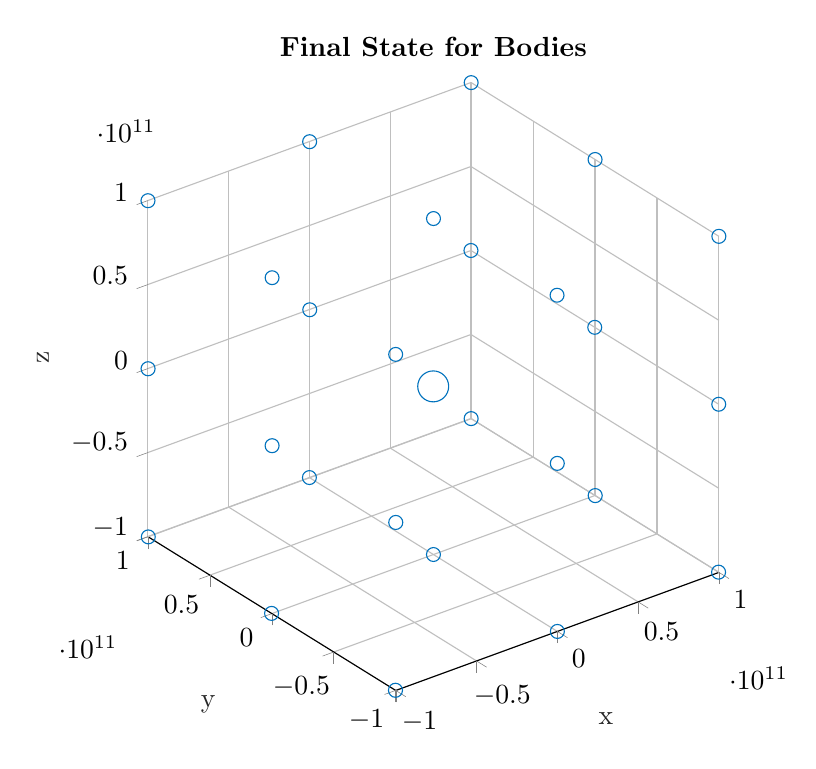
\begin{tikzpicture}

\begin{axis}[%
width=2.856in,
height=3.04in,
at={(0.532in,0.41in)},
scale only axis,
xmin=-100000000000,
xmax=100000000000,
tick align=outside,
xlabel style={font=\color{white!15!black}},
xlabel={x},
ymin=-100099789790,
ymax=100221383780,
ylabel style={font=\color{white!15!black}},
ylabel={y},
zmin=-100000000000,
zmax=100000000000,
zlabel style={font=\color{white!15!black}},
zlabel={z},
view={-37.5}{30},
axis background/.style={fill=white},
title style={font=\bfseries},
title={Final State for Bodies},
axis x line*=bottom,
axis y line*=left,
axis z line*=left,
xmajorgrids,
ymajorgrids,
zmajorgrids,
legend style={at={(1.03,1)}, anchor=north west, legend cell align=left, align=left, draw=white!15!black}
]
\addplot3[scatter, only marks, mark=o, color=mycolor1, mark options={}, scatter/use mapped color=mycolor1, visualization depends on={\thisrow{size} \as \perpointmarksize}, scatter/@pre marker code/.append style={/tikz/mark size=\perpointmarksize}] table[row sep=crcr]{%
x	y	z	size\\
-99997680035	-99855857673	-99997638019	2.53722289127305\\
-99995820981	-100078368310	-58635.022346	2.53722289127305\\
-99997695110	-100009034110	99997623812	2.51246890528022\\
-99995843643	226503275.05	-99995779505	2.52487623459052\\
-99988412223	-179555862.51	-32819.532687	2.52487623459052\\
-99995844851	-181718398.34	99995769983	2.5\\
-99997702127	99812198113	-99997628815	2.51246890528022\\
-99995834363	100002281340	28394.932892	2.53722289127305\\
-99997688220	100066622950	99997631716	2.52487623459052\\
-38982.610169	-100099789790	-99995805526	2.52487623459052\\
-48117.853869	-100038411320	-32185.880326	2.52487623459052\\
24109.366574	-99841676469	99995788472	2.51246890528022\\
11726.151807	12985306.256	-99988385554	2.51246890528022\\
-28519.319386	195477542.09	-15684.045798	5.59016994374947\\
27742.353864	-21179197.996	99988377381	2.51246890528022\\
8934.5609253	100197328670	-99995811305	2.51246890528022\\
-45136.404472	99925853996	17134.979224	2.51246890528022\\
-37145.860615	100011674450	99995806820	2.52487623459052\\
99997669088	-99781825884	-99997684828	2.52487623459052\\
99995807964	-99925688910	4436.776345	2.51246890528022\\
99997695013	-100027683570	99997681472	2.52487623459052\\
99995838034	-135798071.12	-99995820437	2.53722289127305\\
99988403193	228679228.99	-16782.459343	2.51246890528022\\
99995842575	-30315078.36	99995814229	2.52487623459052\\
99997700542	100089944940	-99997679122	2.52487623459052\\
99995828402	100221383780	-17685.690958	2.52487623459052\\
99997679305	100068347900	99997674675	2.51246890528022\\
};
\end{axis}
\end{tikzpicture}
\end{document}